\section{Hardware}
% NOTE: The easiest way to find the hardware specifics of a device
%       is to run the deviceQuery executable (cuda-samples)
%   git clone https://github.com/NVIDIA/cuda-samples.git
%   cd cuda-samples
%   make -j 6
%   cd bin/x86_64/linux/release
%   ./deviceQuery


% NOTE 2:
%  Ampere A100:
%    https://images.nvidia.com/aem-dam/en-zz/Solutions/data-center/nvidia-ampere-architecture-whitepaper.pdf
%    https://developer.nvidia.com/blog/nvidia-ampere-architecture-in-depth/

%  Hopper H100:
%    https://developer.nvidia.com/blog/nvidia-hopper-architecture-in-depth/

%  Blackwell B100:
%    https://resources.nvidia.com/en-us-blackwell-architecture

%  Will be succeeded by the Rubin generation (R100/R200)
%    https://blogs.nvidia.com/blog/computex-2024-jensen-huang/

\subsection{Streaming Multiprocessors \& Thread Blocks}
\begin{frame}
	\frametitle{Streaming Multiprocessor (SM) \& Thread Blocks}
\textit{An understanding of the GPU hardware is fundamental for CUDA programming.}
\begin{itemize}
\item Each GPU device contains a set of Streaming Multiprocessors (\textbf{\textcolor{green}{SM}}).\newline
      (newer generation of GPU devices: \#SMs increase (\textbf{\textcolor{blue}{scalability}}))
\item Work i.e. \textbf{\textcolor{green}{blocks of threads}} are distributed on the different SMs\newline
	(\textbf{\textcolor{blue}{load balancing}}) until SMs are \textbf{\textcolor{red}{full}}\footnote{i.e. resources (registers, shared memory, \ldots) are exhausted}.
\item If the work of a block of threads is completed on an SM, a new block is provided (until all work is done).  		
\item Threads with the same thread block run on the \textbf{\textcolor{green}{same SM}}.\newline
	(allows them to communicate using their shared memory \& synchronize).
\item An SM may run several threads blocks at the same time.
\item Threads within the same thread block are alive simultaneously. 
\end{itemize}
\end{frame} 

\begin{frame}
	\frametitle{Examples of hardware currently available at CHPC: Part $1$}
   \begin{itemize}
      % https://developer.nvidia.com/blog/nvidia-ampere-architecture-in-depth/		   
	   \item \texttt{NVIDIA A100-PCIE-40GB} (\texttt{notch}$293$)  %(Jones: 10.07)
         \begin{itemize}
            \item $108$ SMs, $64$ cores/SM, $4$ third-gen tensor cores/SM.
            \item GPU max. clock rate: $1.41$ GHz
            \item max. \#threads/SM: $2048$ 
            \item max. \#blocks/SM : $32$
            \item FP32 cores/SM: $64$
            \item FP64 cores/SM: $32$
         \end{itemize}	

      %	https://developer.nvidia.com/blog/nvidia-hopper-architecture-in-depth/ 
 \item \texttt{NVIDIA H100 SXM5 NVL} (\texttt{grn}$008$) 
         \begin{itemize}
            \item $132$ SMs, $128$ cores/SM, $4$ fourth-gen tensor cores/SM.
            \item GPU max. clock rate: $1.78$ GHz
            \item max. \#threads/SM: $2048$
            \item max. \#blocks/SM : $32$
            \item FP32 cores/SM: $128$
            \item FP64 cores/SM: $64$
         \end{itemize}
   \end{itemize}
\end{frame}	


\subsection{Types of GPU memory}
\begin{frame}
\frametitle{Types of GPU memory} % Jones:11.05 + 13.07
GPU devices have different types of memory:
\begin{itemize}
	\item \textbf{\textcolor{green}{global}} memory: available to \textcolor{blue}{all threads}.
	\item \textbf{\textcolor{green}{shared}} memory: common to \textcolor{blue}{all threads in a block}.\newline
        The shared memory available on an SM is divided among the blocks on the SM.	  
   \item $32$-bit \textbf{\textcolor{green}{registers}}: fast, on-chip memory (exclusive to each thread).\newline
	 $\Rightarrow$ registers per block: (threads per block) $\times$ (registers per thread).  
   \item \textbf{\textcolor{green}{constant}} memory: cached, read-only
\end{itemize}
\textbf{\textcolor{orange}{Advice}}: 
\begin{itemize}
   \item Try to max. use shared memory \& registers.
   \item Due to their limited availabity, their overuse in a block
         may lead to partially occupied/underutilized SMs.
\end{itemize}		
\end{frame}

\begin{frame}
	\frametitle{Examples of hardware currently available at CHPC (Part $2$)}
   \begin{itemize}
      % https://developer.nvidia.com/blog/nvidia-ampere-architecture-in-depth/
	   \item \texttt{NVIDIA A100-PCIE-40GB} (\texttt{notch}$293$)  %(Jones: 7.31)
         \begin{itemize}
            \item global memory: $40326$ MB HBM2
            \item global memory bandwidth: $1555$ GB/s
            \item shared memory/SM: $164$ kB
            \item \#registers/SM: $65536$
            \item constant memory: $64$ kB		    
            \item L1 cache size/SM: $192$ kB 		    
            \item L2 cache size: $40960$ kB
         \end{itemize}		   

 \item \texttt{NVIDIA H100 SXM5 NVL} (\texttt{grn}$008$) 
        \begin{itemize}
            \item global memory: $95357$ MB HBM3
            \item global memory bandwidth: $3000$ GB/s
            \item shared memory/SM: $228$ kB
            \item \#registers/SM: $65536$
            \item constant memory: $64$ kB
            \item L1 cache size/SM: $192$ kB		    
            \item L2 cache size: $61440$ kB
         \end{itemize}
   \end{itemize}
\end{frame} 

% NOTE: 
\begin{frame}
	\frametitle{\texttt{NVIDIA GH100 SMP}} 
    \begin{columns}
	\column{0.50\textwidth}
    \begin{figure}[H]
       \centering
	    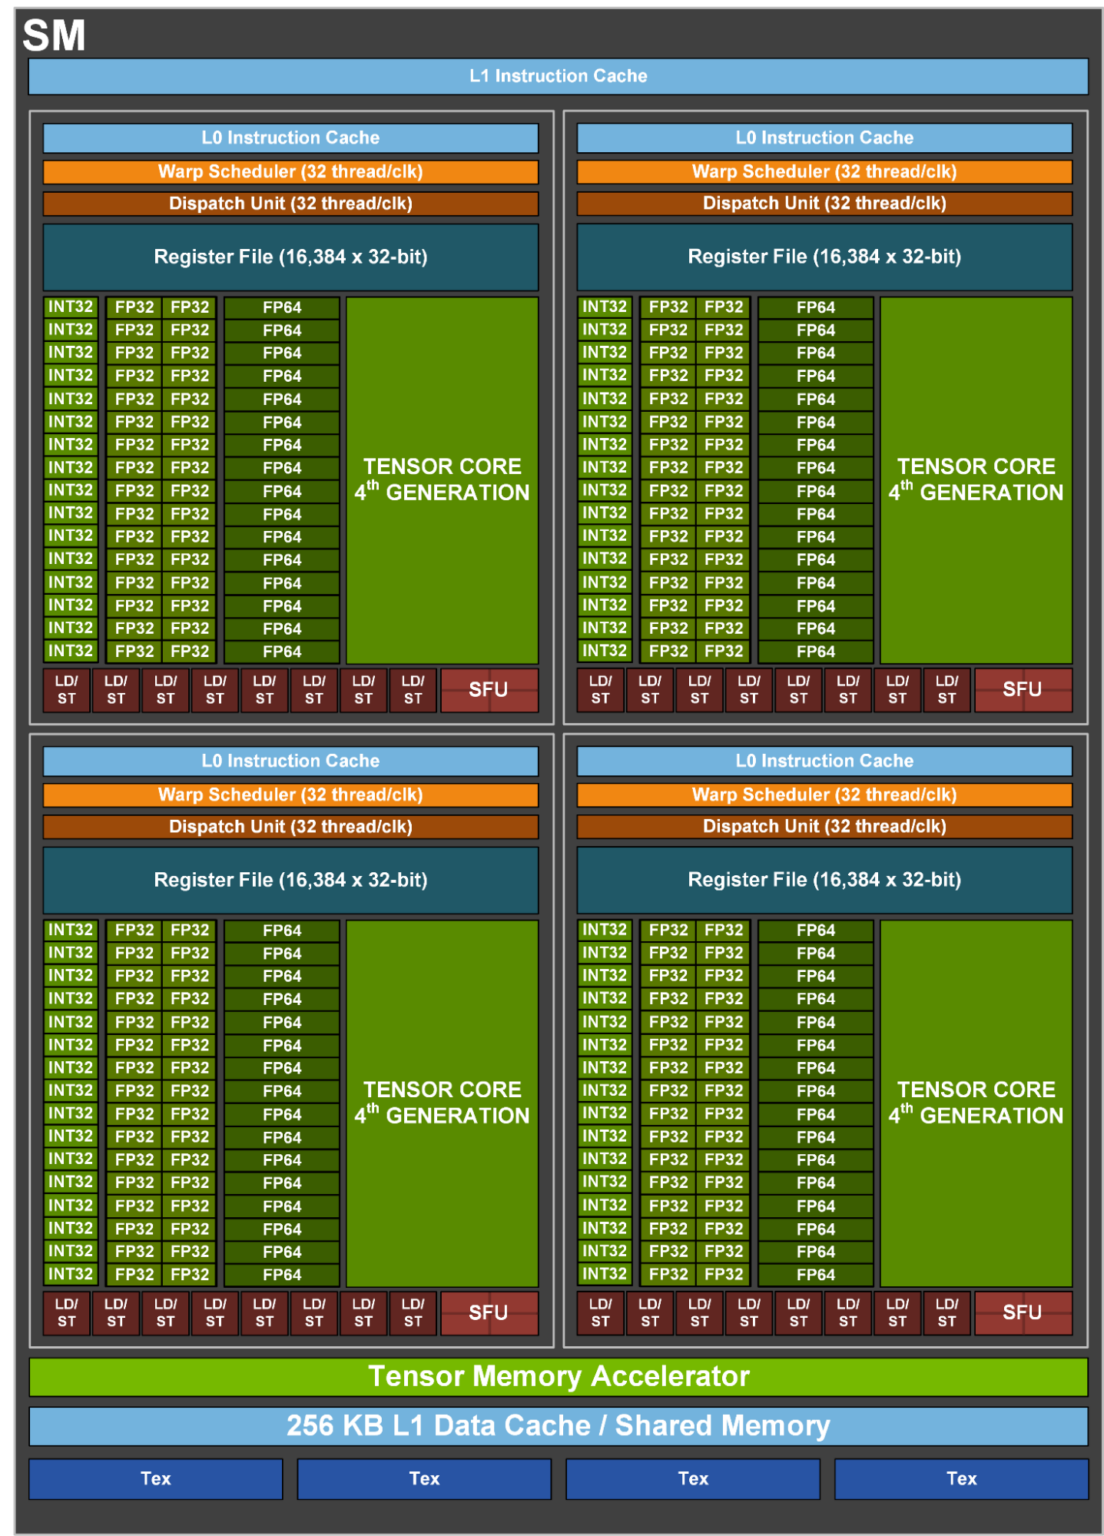
\includegraphics[width=0.80\textwidth]{./img/H100-Streaming-Multiprocessor-SM-1104x1536.png}
	    \caption{\small{GH100 SMP.}}
     \end{figure}
     \end{columns}
\end{frame}

\begin{frame}
        \frametitle{\texttt{NVIDIA GH100 Full Device}}
    \begin{columns}
        \column{0.90\textwidth}
    \begin{figure}[H]
       \centering
	    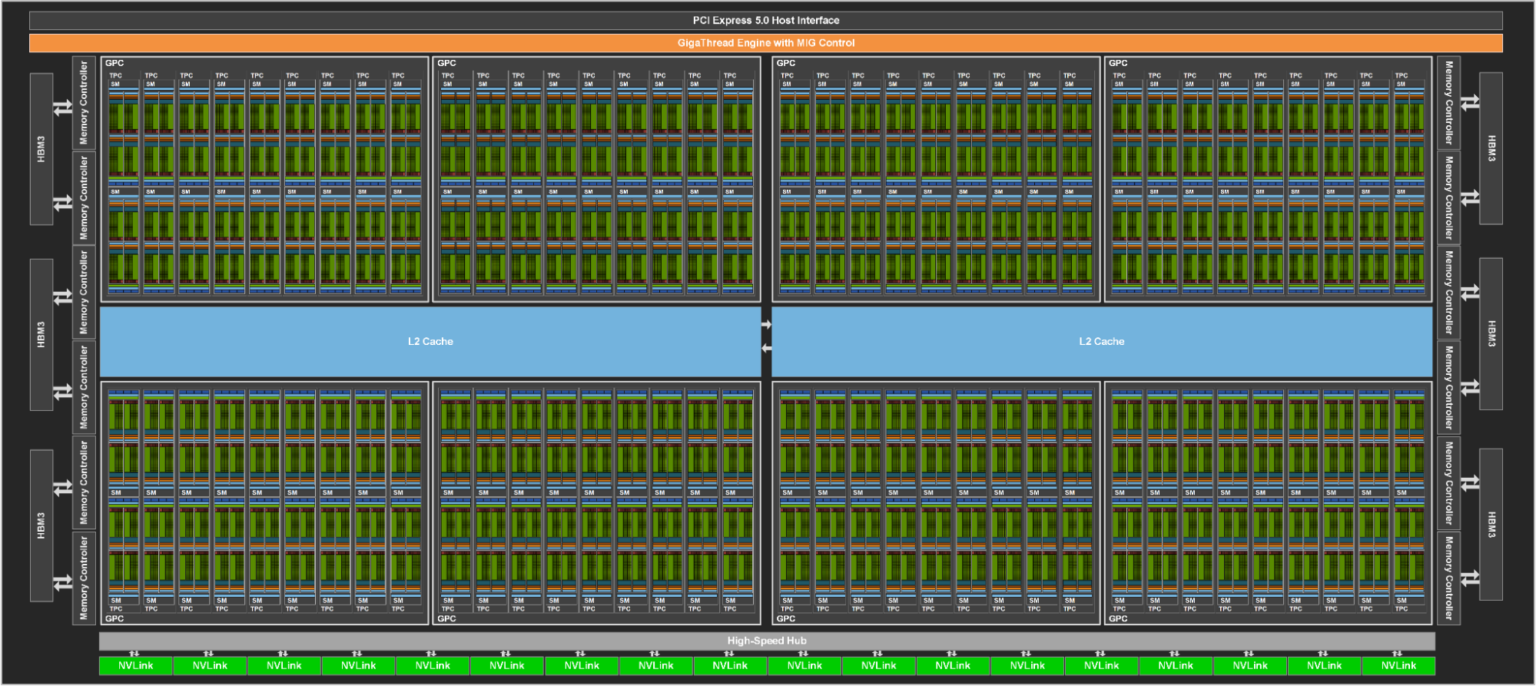
\includegraphics[width=0.90\textwidth]{./img/Full-H100-GPU-with-144-SMs-1536x686.png}
	    \caption{\small{NVIDIA GH100 Full Device ($144$ SMPs).}}
     \end{figure}
     \end{columns}
\end{frame}
